\chapter{Overview of Approach}

We propose a graph based approach for the recommendation task. In this approach a weighted graph of features is used as the model \emph{\Large{M}} and given any query \emph{q}, which contains some part features $p$ we try to find those part features which are close to it. For this we first construct a vocabulary of part features we have including garments and accessories. Next we take a large database of user annotated fashion images and create a co-occurrence graph of various apparels and accessories that are used together in various images by fashionstas. Now given any query item, we pick the $k$--nearest neighbors of the node corresponding to the input item. Here \textit{simrank}\cite{simrank} is used as the similarity measure between nodes to calculate nearest neighbors. In case of more than one items in the input query we generate individual $k$--nearest neighbors lists and then merge the lists using the \textit{Borda's} Rank aggregation algorithm\cite{rankAggregation}. The final aggregated list is recommend to the user. The steps are illustrated in Figure \ref{fig:flowchart}.
\begin{figure}[htb]
\centering
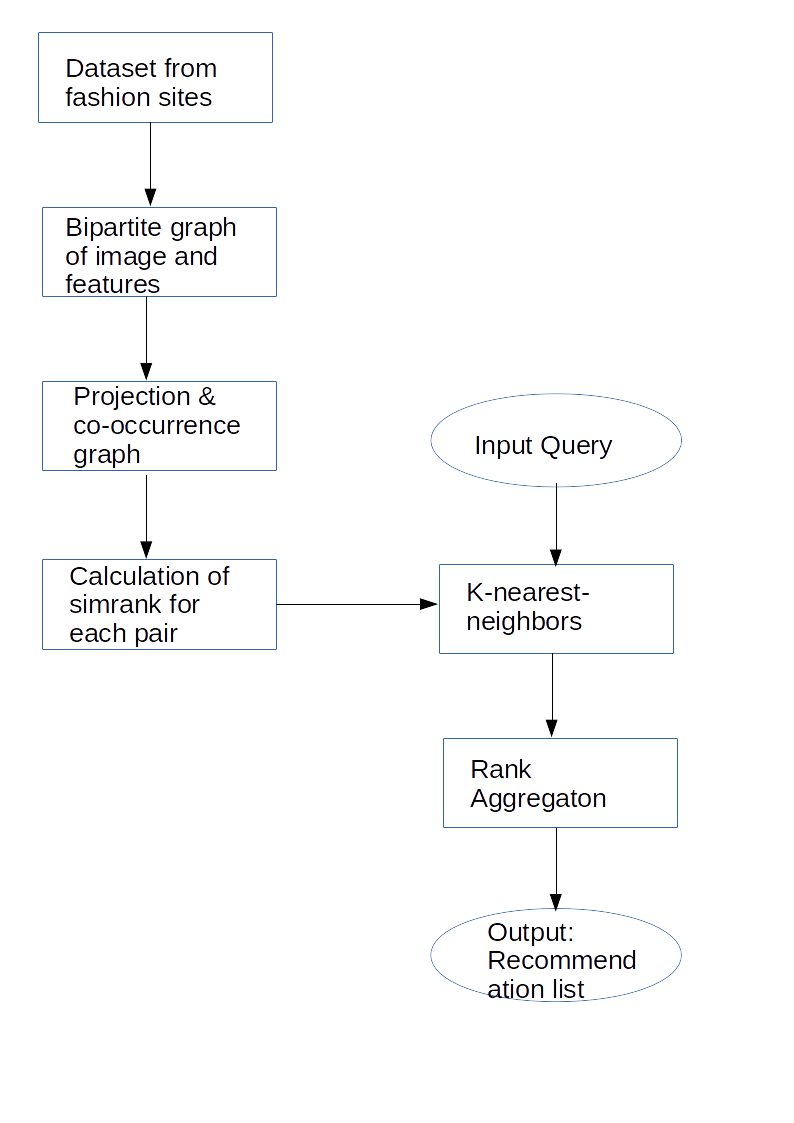
\includegraphics[scale=0.4]{flowchart}
\caption{Flow chart of proposed algorithm.}
\label{fig:flowchart}
\vskip -6pt
\end{figure}


\section{Scrapping Fashion Websites}
As mentioned earlier there are only a handful of public fashion databases available, and finding an annotated fashion dataset is further difficult. But the large number of street fashion images present on the internet and the ease of availability shows immense potential to generate useful user annotated dataset, specially for experiments dealing with contemporary fashion trends. There are various fashion websites where fashionstas upload their images with currently trending apparels, and the images are user annotated i.e. each image is tagged with the type of garments. This makes exactly the kind of dataset we want to work with. We scraped data from a fashion website \url{www.chictopia.com} which is a large style community where bloggers share their style posts and it also has online clothing boutiques. We scraped nearly \textit{500} images of female fashionstas with the tags corresponding to each image. These images cover an appreciable range of street fashion from corporate dressing sense to the most casual of the dresses.

Once the data was scraped we created a vocabulary of part features we had from the database. We used category-description pair as part feature in our work. We had to normalize the tags associated with each image manually because each user used different types of tags. As we are working with \textit{textual} features instead of visual features, this was one necessary step. For each image $P_i$, each part feature $p_j$ has two tags, first is the type of clothing, like shirt, top, etc. and second is its one word description, mostly color. Once this was done we ended up with a codebook of total of \textit{48} unique categories including garments like tops, jeans, etc. and accessories like watches, bracelets, etc. and \textit{632} unique items i.e. category-description pair. For each image, each part is described by a 2--tuple \textit{\{Cloth -- type:Cloth -- description/color\}}. For example \textit{\{Shirt:Blue\}}, \textit{\{Skirt:Black\}}, \textit{\{Watch:Gold\}}, etc. are some valid features in our case.

\section{Simplified Mathematical Formulation}

\subsection{Projection and Co-occurrence graph}

In the dataset, each image $P$ has some part features which is defined using two--tupes as described above. We now have a bipartite graph with dataset images $P$'s as the first partite sets and part features $p_i$'s as the second partite set. There exists an edge between ever part feature and the image in which it occurred. The bipartite graph is then projected to the set of part features. While projecting the graph, simple weighting technique was used, where the weight of an edge between two part features $p_i$ and $p_j$ is the number of common images where $p_i$ and $p_j$ occurred together.

The projected graph so obtained is a weighted co--occurrence graph of the part features. Construction of this graph gives us the relation between different garments and accessories which can be used together and are complementary to each other. The edge weights signify the number of times the part features occurred together i.e. how compatible the garments are when they are worn together. Since the graph is constructed from street fashion images we can safely assume that the co--occurrences are as per the current fashion trends. These are also assumed to be aesthetically sound because they are actually used by models and fashionistas. This step helps us learn a correlation and inter-dependence between various part features from the dataset.

\subsection{Similarity Measure and Nearest Neighbour Consensus}

The co-occurrence graph falls in a domain where nodes represents the objects and edges represents the relations between them. Now we need a similirity measure between the nodes so that we can decide which part feature, or garment in a broader sense, is complementary to which other part features. SimRank\cite{simrank} is an algorithm for analysing the logical graphs and comparing similarity scores between nodes(objects) based on \textit{structural context} in which they appear. We first convert the co--occurrence graph into a directed graph where each edge between part features $p_a$ and $p_b$ in the original graph is replaced by two directed edges $p_a \rightarrow p_b$ and $p_b \rightarrow p_a$ both with weights equal to the weight of original edge. Now we compute \textit{simrank} between each pair of nodes. For fast computation, we leverage the fact that simrank is defined recursively and use \textit{memoization} technique to reduce computation time.

Now, given any part feature $p$ (corresponding to the garment in user's shopping cart) as query we locate the node corresponding to that part feature in the co--occurrence graph. This can be easily done by storing the relation between textual part feature and corresponding node in co--occurrence graph in a hash table. After the node is located, we find out other nodes which are close to it, i.e. nodes which have highest simrank value with this node. Hence we find out the at most top $k$ such nodes, the $k$--nearest--neighbours. The rationale behind this step is that since the graph had edges between part features that were used together by fashionistas and as the simrank values decrease with increase in node distances, the $k$--nearest--neighbors will be those part features which were frequently used with the selected item and are contemporary to it.

So, we get a list of k part features $p_1, p_2, ... p_k$ which are structurally close to the input feature and thus they can be recommended for the given query part feature.

\subsection{Aggregating Ranked Item Recommendations}

If there is only one item in the shopping cart, then the steps mentioned above will suffice. But if we have multiple items in the shopping cart, we need to perform one more task before the final recommendation. Say we have $j$ part features $p_1, p_2, ... p_j$ as input query, we find out individual $k$--nearest--neighbors for each part feature. Now we have $j$ ranked lists, each with $k$ members, which are recommendation related to each input feature. Our final goal is to provide a single ranked list of recommendations. This is a problem of rank aggregation. There are various heuristic based rank aggregation algorithms in literature. We use \textit{Broda's} aggregation algorithm\cite{rankAggregation} for our algorithm.

\textit{Broda's} method is a proportional method in which it assigns a score corresponding to position in which a part feature appears within each ranked list. In our case, for each list $i$, ${p_a}^i$ is assigned a weight ${B_{p_a}}^i$ = $k$ * fraction of part features in the list appearing below $p_a$. This is because in some cases the list does not have $k$ elements but the maximum score that the top element should get is $k$. The \textit{Broda} score of each element $B_{p_a}$ is the the sum of \textit{Broda} scores for that part feature in all the lists.  Then the sorted list in non-increasing order is the final aggregated ranked list. The primary advantage of using this method in our case is that it is computationally very fast and can be implemented in linear time. Thus we get the aggregated ranked list in case of multiple input part features.

We can recomment the top $k$ elements from this ranked list to the user.

\subsection{Overall Algorithm}
The overall algorithm for recommendation can be summarized as presented in Algorithm \ref{algo:main}.
\begin{algorithm}
\DontPrintSemicolon
\SetAlgoLined\DontPrintSemicolon
\KwIn{A list of part features $P$ containing part features $p_1$, $p_2$,...}
\KwOut{A list of recommended part features}
  \SetKwFunction{main}{main}\SetKwFunction{kNearestNeighbors}{kNearestNeighbors}\SetKwFunction{broda}{broda}
  \SetKwProg{myproc}{Algorithm}{}{}
  \myproc{\main{}}{
  $list of recommendation$ \tcp*{list of lists of features}
  \While{$p_i$ in $P$}{
   	$list$ = \kNearestNeighbors{$p_i$} \;
   	$list of recommendation$.add($list$) \;
  }
  $final list$ = \broda{$list of recommendation$} \;
  \KwRet $final list$\;}{}
  
  \setcounter{AlgoLine}{0}

  \SetKwProg{myproc}{Procedure}{}{}
  \myproc{\kNearestNeighbors{$node$}}{
  $set of neighbors$ = BFS($node$)\;
   	\For{$neighbor \in set of neighbors $}{
        ${\tt calculateSimrank}(node, neighbor)$\;
  }
  \KwRet $k\ nodes\ with\ highest\ simrank\ scores$ \;}
  
  \setcounter{AlgoLine}{0}

  \SetKwProg{myproc}{Procedure}{}{}
  \myproc{\broda{$list of lists$}}{
  $max$ = $list of lists$.get(0).size()\;
  $listFinal$ = $nodes$ from each list in $list of lists$\;
  	\For{$list \in list of lists $}{
       	\For{$i < list.size() $}{
    		assign broda score for node(list($i$))= $max$ - $i$\;
        	update $listFinal$\;
        }
   	}
  \KwRet $10\ elements\ of\ listFinal\ with\ highest\ broda\ scores$ \;}

\caption{{\sc Complete The Look}}
\label{algo:main}
\end{algorithm}

\section{Shortcomings in this approach}
There are a few shortcomings with the approach taken. The first and most important concern is that with the increase in number of nodes or features the size of the graph becomes large and difficult to analyze. Calculation of \emph{SimRank} for the whole graph also becomes computationally expensive. Another important concern is that of out of vocabulary queries. Also the textual tags might not always be enough to represent a fashion accessory or garment. For the implementation purpose an optimized code is required to store the feature graph. \emph{Simrank} should also be pre-calculated and stored for each couple of nodes, because calculation of \emph{SimRank} is recursive and calculating it on each query will be very slow and expensive as well.Also the feature graph learned should be updated frequently with the change in trends in contemporary fashion. Creating a dataset for the learning task by manually tagging each image is a tiresome work. Another issue with this approach is network partitioning. If a node or a bunch of nodes is secluded from the graph, it is not possible to generate the recommendations for those part features.